\chapter{What this is, in plain words}

Imagine you film a short video walking around your living room on Monday. On Friday somebody moves
the armchair, takes away a cardboard box, and leaves a rucksack by the door. You film the room
again.

This project takes those two videos and tells you:

\begin{itemize}
  \item the armchair moved, and roughly how far
  \item the box is gone
  \item a rucksack appeared
  \item the table did not move
\end{itemize}

It also shows this as a three dimensional model you can spin round in a web browser, with the
things that changed picked out in colour. Nobody has to tell it what to look for. It works out the
shape of the room from the videos themselves.

\section{Why that is harder than it sounds}

If you simply compared the two videos frame by frame, almost everything would look different. You
stood in a different spot. You held the phone at a different angle. You walked a slightly different
route. The light changed.

The genuinely hard part is not spotting that something is different. It is being certain that an
empty space means \textbf{the object was taken away} rather than \textbf{I just did not point the
camera there the second time}.

\begin{watch}
A person does this without thinking. A computer has to be told the difference, and most systems get
it wrong: they report everything the camera missed as a change. On real footage, where nobody walks
the identical route twice, that is most of the room.
\end{watch}

That problem is what the whole project is built around, and Chapter~4 explains the two ideas that
solve it.

\section{What goes in}

Two ordinary phone videos of the same room, twenty to sixty seconds each, walked along a similar
route. Nothing else. No special camera, no depth sensor, no markers placed in the room, no
measurements taken by hand.

\begin{figure}[h]
\centering
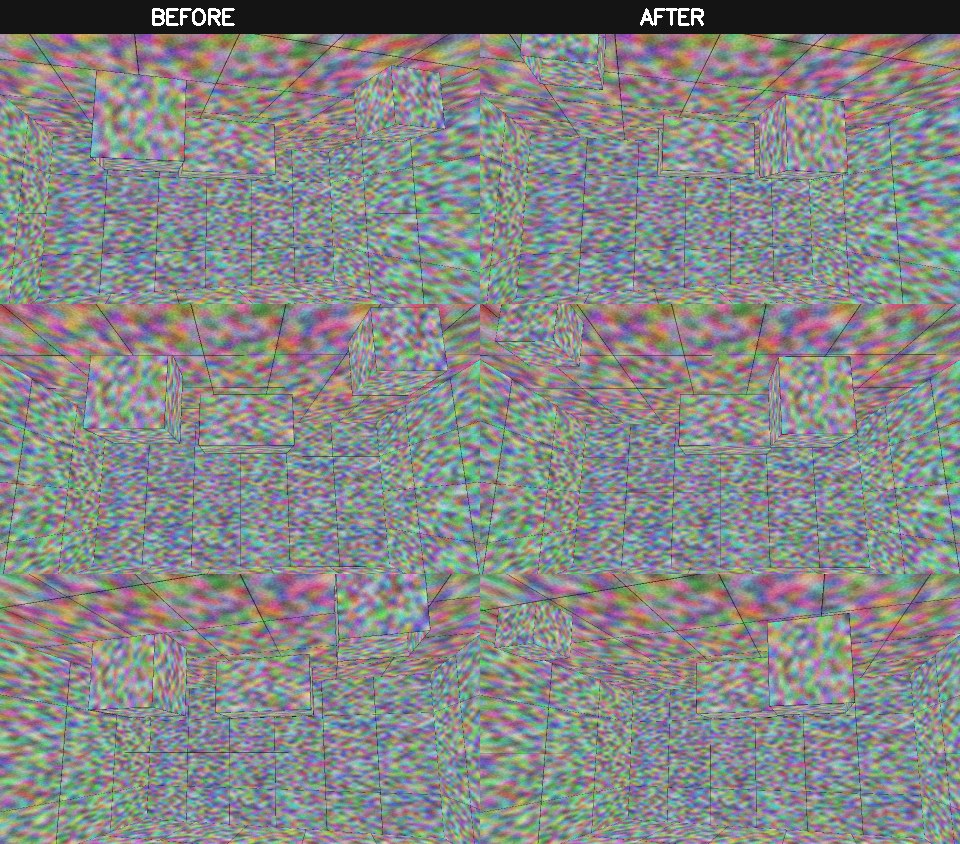
\includegraphics[width=\textwidth]{before_after.jpg}
\caption{Three matching moments from the two recordings used to test the system, before on the left
and after on the right. This is a drawn test room rather than a real one, for reasons explained in
Chapter~6.}
\end{figure}

\section{What comes out}

Three things.

\begin{itemize}
  \item \textbf{An interactive 3D scene} in a web browser. The unchanged room is grey, removals are
        red, additions are green, moves are amber. You can drag to rotate it.
  \item \textbf{A written summary} in ordinary English, for example: ``A chair moved. It was in the
        centre on the left side and is now towards the back on the right side, about 2.4 m away.''
  \item \textbf{A data file} listing every change with its position, size, name and the evidence
        behind the naming, for anything that needs to read the result automatically.
\end{itemize}
